\section{Модификация проекта <<Изображение проекции полиэдра>>}
\subsection*{Постановка задачи}

Пусть точку в пространстве назывется <<хорошей>>, если её проекция находится строго вне квадрата единичной площади с центром в начале координат и сторонами, параллельными координатным осям.   
В данном прокте необходимо было модифицировать эталонный проект таким образом, чтобы определялась и печаталась следующая характеристика полиэдра: сумма длин рёбер, середина и оба из концов которых~--- <<хорошие>> точки.

В общем случае, для успешного решения задачи необходимо знакомство с основами вычислительной геометрии.

\subsection*{Теоретические аспекты}

Для начала приведём некоторые понятия.


\verb|Полиэдр (polyedr)|~--- Множество выпуклых плоских многоугольников. 

\verb|Грань полиэдра (facet)|~--- Выпуклый плоский многоугольник. 

\verb|Ребро полиэдра (edge)|~--- Любая из сторон одной из граней. 

\verb|Вершина полиэдра (vertex)|~--- Любая из вершин произвольной грани. 


\begin{figure}[ht!]
\begin{center}
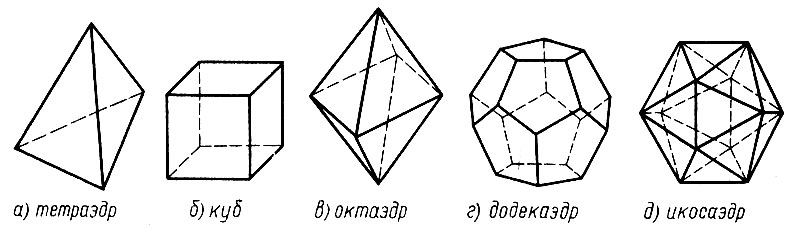
\includegraphics[width=0.9\hsize]{images/poly2}
\end{center}
\caption{Некоторые виды полиэдров}\label{fig:poly2}
\end{figure}


В рассматриваемом проекте речь идёт о геометрических объектах, находящихся в трёхмерном пространстве, поэтому необходимо вспомнить некоторые факты из линейной алгебры и аналитической геометрии.

Прежде всего вследует вспомнить, что точку пространства $\mathbb R^3$ можно задать с помощью трёх действительных чисел~---  её координат. Эти же координаты задают и вектор трёхмерного пространства, начало которого совпадает с началом координат, а конец~---  с рассматриваемой точкой.

Для векторов в пространстве определены операции сложения, вычитания и умножения на число, порождающие новый вектор, координаты которого находятся с помощью сложения, вычитания и умножения на число координат исходных векторов.

Также необходимо знание  скалярного, векторного и смешанного произведения векторов, и уметь использовать данные операции.

 Помимо прочего, в данном проекте необходимо использовать линейные преобразования (отображения) плоскости и пространства. Любое такое преобразование, как известно, задаётся квадратной матрицей порядка два для плоскости и порядка три для пространства. Напомним, что тождественному преобразованию соответствует единичная матрица $E$.

Среди всех преобразований в данном случае особенно интересны повороты и гомотетия, задаваемая матрицей вида $kE,$ где $k$~---  положительная константа, а $E$~---  единичная матрица.  
Ортогональные преобразования плоскости и пространства, сохраняющие ориентацию, являются поворотами. На плоскости поворот на угол $\varphi$ задаётся матрицей вида

\begin{center}
$\begin{pmatrix}\cos\varphi&\sin\varphi\\ -\sin\varphi&\cos\varphi\end{pmatrix}.$
\end{center}.

В случае пространства повороту на угол $\varphi$ вокруг оси $Oz$ соответствует следующая матрица: 
\begin{center}
$\begin{pmatrix}\cos\varphi& \sin\varphi & 0 \\ -\sin\varphi&\cos\varphi& 0\\
0 & 0 & 1\end{pmatrix}.$
\end{center}.

Аналогичный вид имеют и матрицы поворота вокруг осей $Ox$ и $Oy,$ а произвольное вращение пространства может быть представлено в виде композиции трёх последовательных поворотов вокруг осей $Oz, Oy$ и вновь $Oz$.

В процессе работы над проектом нам потребуется решать следующую задачу: найти пересечение отрезка с полупространством, которое задано точкой на граничной плоскости и вектором внешней нормали к ней. Двумерный аналог этой задачи таков: найти пересечение отрезка на плоскости с полуплоскостью, которая задана точкой на граничной прямой и вектором внешней нормали к этой прямой. Рассмотрим решение последней из задач.

Пусть концы отрезка $B$ (от английского слова \verb|begin|) и $F$ (от \verb|final|) имеют соответственно координаты $(x_1, y_1)$ и $(x_2, y_2)$ точка на граничной прямой~---  координаты $(x_0, y_0),$ а вектор внешней нормали к полуплоскости~---  это вектор $\overrightarrow N$.

Для этого необходимо и достаточно, чтобы оба конца отрезка лежали с «нужной» стороны от заданной прямой.

Точка $(x_1, y_1)$ будет лежать с <<нужной>> (внешней по отношению к полуплоскости) стороны от граничной прямой, если угол между векторами внешней нормали и вектором, соединяющим точки $(x_0, y_0)$ и $(x_1, y_1)$ является острым.

Искомое условие имеет следующий вид: $\overrightarrow N \cdot \overrightarrow{AB} > 0.$
Тогда для того чтобы пересечение отрезка с полуплоскостью представляло собой пустое множество, необходимо чтобы:
$\overrightarrow N \cdot\overrightarrow{AB} > 0 \wedge \overrightarrow N \cdot \overrightarrow{AF} > 0$.

Если знаки указанных скалярных произведений разные, то отрезок пересекает прямую, ограничивающую полуплоскость. В этом случае для определения пересечения отрезка с полуплоскостью прежде всего необходимо найти точку их пересечения. Произвольная точка отрезка $BF$ может быть записана как $(1-t)B + tF,$ где $0 \leqslant t \leqslant 1$. При $t = 0$ эта формула задаёт начало отрезка (точку $B$ ), а при $t=1$~---  его конец (точку $F$). Отсюда следует, что искомая точка пересечения в свою очередь соответствует значению  $$t = \frac{\overrightarrow N \cdot \overrightarrow{AB}} {\overrightarrow N \cdot \overrightarrow{AF} - \overrightarrow N \cdot \overrightarrow{AB}},$$ так как для неё $\overrightarrow N \cdot \overrightarrow{AC} = 0$.
 
\subsection*{ Описание используемых структур и применяемых алгоритмов}

Точку в трёхмерном пространстве ($\mathbb R^3$), так же, как и вектор этого пространства, мы будем представлять объектом класса \verb|R3|, имеющем три действительные компоненты (\verb|@x, @y| и \verb|@z|),~---  координаты точки или вектора. В этом классе реализуем ряд методов, обеспечивающих все необходимые в данном проекте манипуляции над точками  (векторами).

Каждое из рёбер (экземпляров класса \verb|Edge|) полиэдра будем задавать его началом и концом~---  объектами класса \verb|R3|, а произвольную его грань (экземпляр класса \verb|Facet|)~---  массивом её вершин. Сам полиэдр будет являться экземпляром класса \verb|Polyedr|, в конструкторе (методе \verb|initialize|) которого будет обрабатываться файл, содержащий всю информацию о полиэдре.

Так как плоскость проектирования горизонтальна, то достаточно <<забыть>> $z$-координату.

Теперь рассмотрим некоторые программистские аспекты. Модификация данного проекта довольна проста и, по сути, заключается в добавлении нового параметра~---  суммы длин рёбер, середина и оба из концов которых~---  «хорошие» точки. Следовательно  вся задача сводится к определению <<хороших>> точек ребра и  умению вычислять середину отрезка.

Найдем обратное условие, когда данная нам точка не является  <<хорошей>>. Очевидно, что оно будет выглядеть  следующим образом (так как мы рассматриваем проекцию ~---  нет смысла включать в условие координату  \verb|z|):
\begin{center}
 $x,y < 0.5$ & $x,y > -0.5$
\end{center}

 
Учитывая коэффициент гомотетии и данное условие, можно написать необходимый метод:
\begin{lstlisting}
def good?(c)
   return false if ((@x.abs<0.5*c)&&(@y.abs<0.5*c))
   true
end
\end{lstlisting}

Середина отрезка находится стандартным способом:

Пусть заданы два конца отрезка в пространстве $A(x_a,y_a,z_a)$ и $B(x_b,y_b,z_b),$ тогда середина отрезка имеет следующие координаты:

 $$x_c = \frac {x_a+x_b}2, \ y_c = \frac {y_a+y_b}2, \ z_c = \frac {z_a+z_b}2.$$
 

Для реализации данного метода у класса  \verb|Edge|(Ребро) есть две переменные  \verb|@@beg|, \verb|@@fin|, отвечающие за начало и конец отрезка.  Учитывая то, что каждая из этих точек уже имеет свои координаты, метод нахождения середины отрезка будет выглядеть следующим образом:  

\begin{lstlisting}
def middle
   (@beg+@fin)/2
end
\end{lstlisting}

Исходя из всего вышеупомянутого, можно написать метод вычисления длины ребра. Чтобы найти длину отрезка можно воспользоваться скалярным произведением векторов. Для этого необходимо ребро превратить в вектор, то есть взять разность \verb|@fin-@beg|, обозначить её как  $\vec A,$  и используя метод класса  \verb|R3 dot|, вычислить квадратный  корень из скалярного квадрата вектора  $\vec A$.  Ниже представлена реализация методов \verb|dot|  и \verb|length|.
\begin{lstlisting}
def dot(other) 
   @x*other.x+@y*other.y+@z*other.z
end
\end{lstlisting}


\begin{lstlisting}
def length(c)
   if (@beg.good?(c) && @fin.good?(c) && self.middle)
     a=(@fin-@beg)*(1/c)
     Math.sqrt(a.dot(a))
   else
     0
   end
end 
\end{lstlisting}


Итак, всё что остаётся сделать~--- при задании нового ребра его вершинами, проверять координаты начала, конца и середины ребра на <<хорошие>> точки, и суммировать подходящие нам рёбра. Всё это реализуется в классе \verb|Polyedr|,  в цикле задания рёбер очередной грани:


\begin{lstlisting}
(0...size).each do|n| 
     e = Edge.new(vertexes[n-1],vertexes[n])
     @edges << e
     @length += e.dist(c)
end
\end{lstlisting}



